\documentclass[manuscript, review, nonacm]{acmart}

% --- PACKAGES ---
\usepackage{graphicx}
\usepackage{booktabs}
\usepackage{amsmath}
\usepackage{subcaption}
\usepackage{siunitx}
\usepackage{url}
\usepackage{tikz}
\usetikzlibrary{positioning, arrows.meta, shapes.geometric, calc}

% --- LATEX TWEAKS FOR SPACE SAVING ---
\setlength{\textfloatsep}{8pt plus 1.0pt minus 2.0pt}
\setlength{\floatsep}{8pt plus 1.0pt minus 2.0pt}
\setlength{\intextsep}{8pt plus 1.0pt minus 2.0pt}
\setlength{\abovedisplayskip}{3pt}
\setlength{\belowdisplayskip}{3pt}

% ============================================================
% RESULTS PLACEHOLDERS — fill from results/*.csv after the server retrain.
% Convention: each cell is a macro holding "mean" and a second holding "std".
% Values marked TBD await the corrected-env retraining run; the others are the
% heuristic numbers already measured (20 seeds), which are unaffected by the
% switching-cost fix in the static/dynamic scenarios.
% ============================================================
\newcommand{\Nseed}{20}
% --- Static scenario (mean / std over \Nseed seeds) ---
\newcommand{\DRLstatM}{4374}\newcommand{\DRLstatS}{1141}
\newcommand{\GreStatM}{4390}\newcommand{\GreStatS}{1145}
\newcommand{\HybStatM}{4380}\newcommand{\HybStatS}{1144}
\newcommand{\RndStatM}{-417}\newcommand{\RndStatS}{429}
% --- Dynamic scenario ---
\newcommand{\DRLdynM}{3972}\newcommand{\DRLdynS}{1087}
\newcommand{\GreDynM}{4029}\newcommand{\GreDynS}{1082}
\newcommand{\HybDynM}{4020}\newcommand{\HybDynS}{1077}
\newcommand{\RndDynM}{-1427}\newcommand{\RndDynS}{336}
% --- Realistic scenario (cost = 2 min, corrected dynamics) ---
\newcommand{\DRLrealM}{495}\newcommand{\DRLrealS}{544}
\newcommand{\GreRealM}{2044}\newcommand{\GreRealS}{634}
\newcommand{\HybRealM}{2039}\newcommand{\HybRealS}{630}
\newcommand{\RndRealM}{-32}\newcommand{\RndRealS}{71}
% --- Headline relative performance of DRL vs Greedy in the Realistic scenario ---
\newcommand{\DRLrealRel}{24.2\%}
% --- Switching-cost collapse threshold (minutes) observed in the ablation ---
\newcommand{\CollapseCost}{5}

\begin{document}

\title{An Empirical Study of Deep Reinforcement Learning for Dynamic Scheduling in Satellite QKD Networks}

\author{Phuc Hao Do}
\orcid{0000-0003-0645-0021}
\affiliation{\institution{Danang Architecture University} \city{Da Nang} \country{Viet Nam}}
\email{haodp@dau.edu.vn}
\affiliation{\institution{The Bonch-Bruevich Saint Petersburg State University of Telecommunications} \city{Saint Petersburg} \country{Russia}}
\email{do.hf@sut.ru}

\begin{abstract}
Efficiently scheduling links for satellite-based Quantum Key Distribution (QKD) networks is critical for global secure communication, yet it remains challenging under dynamic orbital and atmospheric conditions. This letter investigates the efficacy of Deep Reinforcement Learning (DRL) for this task by training a Proximal Policy Optimization agent across three simulation environments of increasing realism: \textit{Static}, \textit{Dynamic} (with cloud disruptions), and \textit{Realistic} (with link-switching costs). To keep the comparison fair, every policy is scored by the same physical objective, the total secure key generated over a 24-hour horizon, and all results are reported as the mean and standard deviation over \Nseed{} independent seeds. Our central finding is counterintuitive: although DRL matches a strong domain-aware greedy heuristic in the simpler settings, it fails to outperform that heuristic once realistic switching costs are introduced, even after three million training steps. We further show, through a switching-cost sensitivity analysis and a cost-aware hybrid baseline, that the gap is driven by the structure of the problem rather than by insufficient training. The study provides a reproducible benchmark and a cautionary case for the practical deployment of DRL in cost-aware network scheduling.
\end{abstract}

\begin{CCSXML}
<ccs2012>
   <concept><concept_id>10010147.10010257.10010258.10010261</concept_id><concept_desc>Computing methodologies~Reinforcement learning</concept_desc><concept_significance>500</concept_significance></concept>
   <concept><concept_id>10002978.10003022.10003023</concept_id><concept_desc>Security and privacy~Quantum cryptography</concept_desc><concept_significance>500</concept_significance></concept>
</ccs2012>
\end{CCSXML}
\ccsdesc[500]{Computing methodologies~Reinforcement learning}
\ccsdesc[500]{Security and privacy~Quantum cryptography}
\keywords{Deep Reinforcement Learning, QKD, Satellite Networks, Scheduling}

\maketitle

\section{Introduction}\label{sec:introduction}
The demand for unconditionally secure communication has positioned Satellite-based Quantum Key Distribution (Sat-QKD) as a vital technology for a global quantum network \cite{gisin2002quantum, liao2017satellite}. A single low Earth orbit (LEO) satellite can distribute keys to many optical ground stations (OGS), but only one downlink can be served at a time, so the network operator must decide, minute by minute, which OGS to serve. This is a genuine network-level scheduling problem: the controller manages a shared, fast-moving resource across competing ground nodes, and its decisions determine the aggregate secure key delivered to the network. The decision is complicated by orbital mechanics \cite{deniz2021routing}, by unpredictable atmospheric disruptions such as cloud cover \cite{bourgoin2013comprehensive}, and by the operational cost of reconfiguring a link, all of which render static or simple greedy strategies potentially suboptimal \cite{oi2021optimization}. Deep Reinforcement Learning (DRL) offers a model-free framework for exactly this class of sequential control problems \cite{sutton2018reinforcement}, which motivates a careful study of whether it delivers a practical advantage here.

In this letter, we present a rigorous empirical study of DRL for Sat-QKD scheduling\footnote{Source code: \url{https://github.com/ailabteam/AILET}}. Our contributions are threefold. First, we formulate the task as a Markov Decision Process with an explicit, fully specified reward and evaluate all policies under one identical physical objective, so the comparison cannot be biased by reward design. Second, we benchmark a Proximal Policy Optimization (PPO) agent against a strong greedy heuristic, a cost-aware hybrid heuristic, and a random lower bound across three environments of increasing realism, reporting mean and standard deviation over \Nseed{} seeds. Third, we sweep the link-switching cost to show both why the learned agent struggles and where scheduling becomes infeasible for every policy. We find that DRL does not outperform the greedy heuristic once switching costs are present, even after three million steps, and that the cost-aware hybrid does not close the gap because most reconfigurations are forced by orbital geometry rather than chosen.

\section{Problem Formulation}\label{sec:formulation}
We model the task as a Markov Decision Process (MDP) defined by the tuple $(\mathcal{S}, \mathcal{A}, \mathcal{P}, \mathcal{R}, \gamma)$ \cite{sutton2018reinforcement}. The agent learns a policy $\pi_\theta(a\,|\,s)$ that maximizes the expected discounted return
\begin{equation}
J(\pi_\theta) = \mathbb{E}_{\pi_\theta}\!\left[\, G_t \,\right], \qquad
G_t = \sum_{k=0}^{\infty} \gamma^{k}\, r_{t+k+1}, \quad \gamma \in [0,1].
\label{eq:return}
\end{equation}
The episode spans a 24-hour horizon discretized at $\Delta t = \SI{60}{\second}$, giving $T = 1440$ steps. We instantiate the components as follows.

\textbf{State space ($\mathcal{S}$).} At step $t$ the agent observes a normalized vector $s_t = s_t^{\text{sat}} \oplus s_t^{\text{ogs}} \oplus s_t^{\text{scn}} \in [-1,1]^{D}$. The base block $s_t^{\text{sat}} \in \mathbb{R}^4$ encodes the minute of day $m_t$ and the satellite sub-point $(\phi_t,\lambda_t,h_t)$ obtained by propagating its TLE set \cite{vallado2001fundamentals},
\begin{equation}
s_t^{\text{sat}} = \Big(\tfrac{m_t}{720}-1,\; \tfrac{\phi_t}{90^\circ},\; \tfrac{\lambda_t}{180^\circ},\; \tfrac{h_t}{\SI{1000}{\km}}\!\cdot 2 - 1\Big).
\label{eq:statesat}
\end{equation}
For each ground station $i$ we form the topocentric link geometry from the slant vector $\mathbf{r}_{t,i} = \mathbf{p}^{\text{sat}}_t - \mathbf{p}^{\text{ogs}}_i$, yielding elevation $e_{t,i}$, azimuth $\alpha_{t,i}$, and slant range $d_{t,i}=\lVert \mathbf{r}_{t,i}\rVert$. The per-station feature is gated by visibility,
\begin{equation}
v_{t,i} =
\begin{cases}
\big(\tfrac{e_{t,i}}{90^\circ},\; \tfrac{\alpha_{t,i}}{180^\circ}-1,\; 1-\tfrac{d_{t,i}}{d_{\max}}\big), & e_{t,i} \ge \theta_{\min},\\[2pt]
(-1,-1,-1), & \text{otherwise},
\end{cases}
\label{eq:statelink}
\end{equation}
with $\theta_{\min}=\SI{20}{\degree}$ and $d_{\max}=\SI{4000}{\km}$, and $s_t^{\text{ogs}} = \oplus_{i=1}^{N_{\text{ogs}}} v_{t,i}$. The scenario block $s_t^{\text{scn}}$ appends the normalized cloud-cover vector $c_t/c_{\max}$ (Dynamic, Realistic) and the normalized link-setup timer $\tau_t/C$ (Realistic), so $D$ grows from $4+3N_{\text{ogs}}$ to $5+4N_{\text{ogs}}$.

\textbf{Action space ($\mathcal{A}$).} A discrete space $\mathcal{A}=\{0,\dots,N_{\text{ogs}}\}$, where $a_t=i<N_{\text{ogs}}$ attempts a connection with $\text{OGS}_i$ and $a_t=N_{\text{ogs}}$ is the \textit{idle} action, directly compatible with PPO \cite{schulman2017proximal}.

\textbf{Secure-key channel model.} For a valid connection, the downlink is dominated by free-space optical path loss \cite{liao2017satellite, bourgoin2013comprehensive}. We express the loss in decibels, convert to a transmittance $\eta_{t,i}$, and scale a nominal raw rate to obtain the secure key produced in one step,
\begin{align}
L_{t,i} &= L_0 + 20\log_{10}\!\big(d_{t,i}/d_{\text{ref}}\big) \quad [\si{\decibel}], \label{eq:pathloss}\\
\eta_{t,i} &= 10^{-L_{t,i}/10}, \qquad
K_{t,i} = R_0\,\eta_{t,i}\,\Delta t, \label{eq:keyrate}
\end{align}
with reference distance $d_{\text{ref}}=\SI{1000}{\km}$, fixed loss $L_0=\SI{50}{\decibel}$, and raw rate $R_0=\SI{e5}{bits\per\second}$. Eq.~\eqref{eq:pathloss} makes the elevation angle the physically dominant driver of throughput, since higher elevation shortens the slant range $d_{t,i}$.

\textbf{Switching-cost dynamics.} A reconnection to a different station incurs a setup latency during which no key flows. Let the switch indicator be $\sigma_t = \mathbb{1}[\,a_t \neq a_{t-1} \wedge a_t \neq N_{\text{ogs}}\,]$. The setup timer is armed on a switch and counted down afterwards,
\begin{equation}
\tau_t^{+} = \begin{cases} C, & \sigma_t = 1,\\ \tau_t, & \sigma_t = 0,\end{cases}
\qquad
\tau_{t+1} = \max\!\big(\tau_t^{+}-1,\,0\big),
\label{eq:timer}
\end{equation}
so a nominal cost of $C$ minutes forfeits exactly $C$ steps of potential key (we use $C=2$).

\textbf{Reward.} Combining the channel model, the constraints, and the setup state gives
\begin{equation}
r_{t+1} =
\begin{cases}
0, & \tau_t^{+} > 0 \;\;\text{(in link setup),}\\
0, & a_t = N_{\text{ogs}} \;\;\text{(idle),}\\
-5, & \text{$\text{OGS}_{a_t}$ cloud-blocked,}\\
-1, & e_{t,a_t} < \theta_{\min},\\
K_{t,a_t}, & \text{otherwise (valid connection).}
\end{cases}
\label{eq:reward}
\end{equation}
One point is essential for a fair reading of our results: the scalar in Eq.~\eqref{eq:reward} is the \emph{single physical objective used to score every policy}, the learned agent and all baselines alike. No policy is evaluated against a private or differently weighted reward, so any performance gap reflects scheduling quality rather than reward shaping. The agent-environment loop is shown in Figure~\ref{fig:system_diagram}.

\begin{figure}[t]
  \centering
  \resizebox{\linewidth}{!}{%
  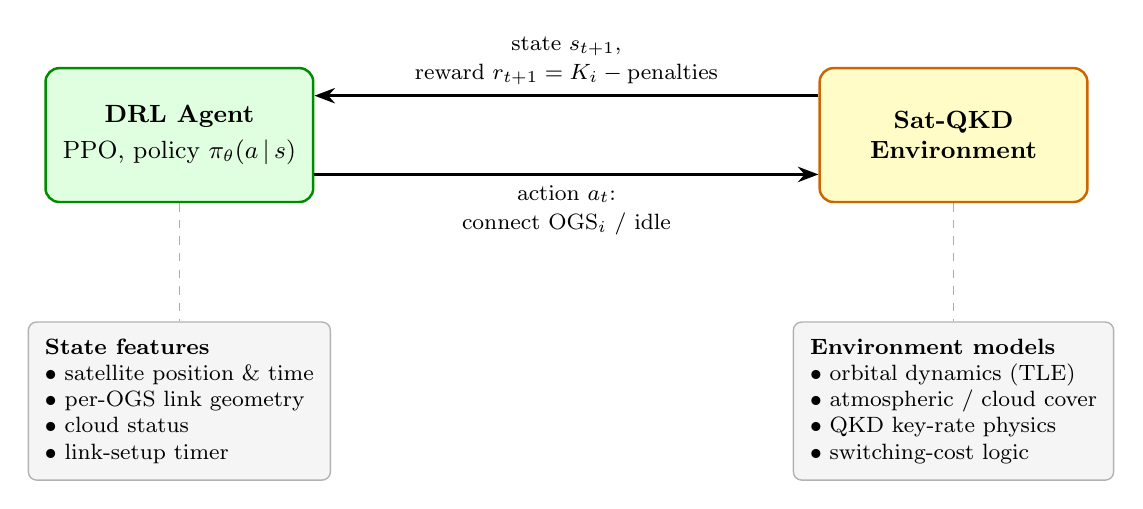
\begin{tikzpicture}[
    font=\small,
    >={Stealth[length=2.6mm]},
    agentstyle/.style={rounded corners=5pt, draw=green!55!black, fill=green!12,
        text=black, line width=0.9pt, minimum width=3.4cm, minimum height=1.7cm, align=center},
    envstyle/.style={rounded corners=5pt, draw=orange!80!black, fill=yellow!22,
        text=black, line width=0.9pt, minimum width=3.4cm, minimum height=1.7cm, align=center},
    detailstyle/.style={rounded corners=3pt, draw=gray!60, fill=gray!8, text=black,
        line width=0.5pt, align=left, font=\footnotesize, inner sep=6pt},
    flow/.style={->, line width=1.1pt},
    link/.style={dashed, draw=gray!65, line width=0.6pt}
  ]
    \node[agentstyle] (agent) {\textbf{DRL Agent}\\[2pt]PPO, policy $\pi_\theta(a\,|\,s)$};
    \node[envstyle, right=6.4cm of agent] (env) {\textbf{Sat-QKD}\\\textbf{Environment}};
    % state + reward: environment -> agent (upper)
    \draw[flow] ([yshift=5mm]env.west) -- node[above, align=center, font=\footnotesize]
        {state $s_{t+1}$,\\[1pt] reward $r_{t+1}=K_i-\text{penalties}$}
        ([yshift=5mm]agent.east);
    % action: agent -> environment (lower)
    \draw[flow] ([yshift=-5mm]agent.east) -- node[below, align=center, font=\footnotesize]
        {action $a_t$:\\[1pt] connect OGS$_i$ / idle}
        ([yshift=-5mm]env.west);
    \node[detailstyle, below=1.5cm of agent] (sdet)
        {\textbf{State features}\\
         $\bullet$ satellite position \& time\\
         $\bullet$ per-OGS link geometry\\
         $\bullet$ cloud status\\
         $\bullet$ link-setup timer};
    \node[detailstyle, below=1.5cm of env] (edet)
        {\textbf{Environment models}\\
         $\bullet$ orbital dynamics (TLE)\\
         $\bullet$ atmospheric / cloud cover\\
         $\bullet$ QKD key-rate physics\\
         $\bullet$ switching-cost logic};
    \draw[link] (agent.south) -- (sdet.north);
    \draw[link] (env.south) -- (edet.north);
  \end{tikzpicture}}
  \caption{The Sat-QKD scheduling loop as an MDP. At each step the agent observes the state (satellite position, per-OGS link geometry, cloud status, and the link-setup timer), selects which ground station to serve, and receives the secure key rate of Eq.~\eqref{eq:keyrate} net of operational penalties. The environment captures orbital, atmospheric, physical, and operational dynamics.}
  \label{fig:system_diagram}
\end{figure}

\section{Experimental Setup}\label{sec:setup}
Our simulation features one LEO satellite and five OGSs over a 24-hour episode. We evaluate three scenarios of increasing realism, summarized in Figure~\ref{fig:scenarios}: a \textit{Static} environment testing geometric optimization; a \textit{Dynamic} environment adding time-correlated cloud cover, which forces reactive avoidance; and a \textit{Realistic} environment adding the two-minute link-switching cost of Eq.~\eqref{eq:reward}, which requires cost-aware planning.

\begin{figure}[t]
  \centering
  \resizebox{\linewidth}{!}{%
  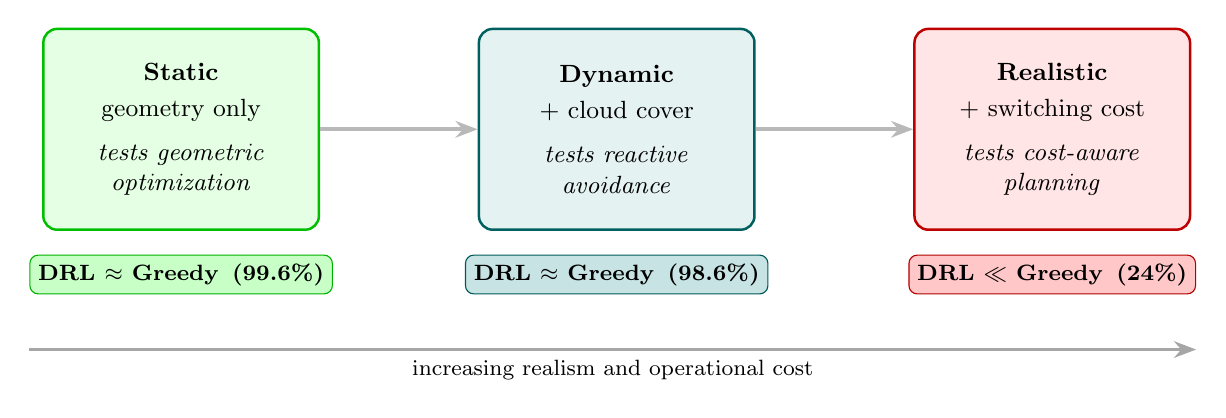
\begin{tikzpicture}[
    font=\small,
    >={Stealth[length=2.8mm]},
    scen/.style={rounded corners=5pt, draw=#1!75!black, fill=#1!10, text=black,
        line width=0.9pt, minimum width=3.5cm, minimum height=2.55cm,
        align=center, inner sep=5pt},
    badge/.style={rounded corners=3pt, fill=#1!22, draw=#1!70!black, text=black,
        font=\footnotesize\bfseries, inner sep=3pt},
    escalate/.style={->, line width=1.4pt, draw=gray!55}
  ]
    \node[scen=green] (s1) {\textbf{Static}\\[2pt]geometry only\\[5pt]\textit{tests geometric}\\ \textit{optimization}};
    \node[scen=teal, right=2.0cm of s1] (s2) {\textbf{Dynamic}\\[2pt]$+$ cloud cover\\[5pt]\textit{tests reactive}\\ \textit{avoidance}};
    \node[scen=red, right=2.0cm of s2] (s3) {\textbf{Realistic}\\[2pt]$+$ switching cost\\[5pt]\textit{tests cost-aware}\\ \textit{planning}};
    \draw[escalate] (s1.east) -- (s2.west);
    \draw[escalate] (s2.east) -- (s3.west);
    \node[badge=green, below=3mm of s1] (b1) {DRL $\approx$ Greedy\, (99.6\%)};
    \node[badge=teal,  below=3mm of s2] (b2) {DRL $\approx$ Greedy\, (98.6\%)};
    \node[badge=red,   below=3mm of s3] (b3) {DRL $\ll$ Greedy\, (24\%)};
    \coordinate (railL) at ($(b1.south west)+(0,-0.7)$);
    \coordinate (railR) at ($(b3.south east)+(0,-0.7)$);
    \draw[->, line width=1.2pt, draw=gray!70] (railL) -- (railR) node[midway, below, font=\footnotesize] {increasing realism and operational cost};
  \end{tikzpicture}}
  \caption{Experimental design: three scenarios of increasing realism and the headline outcome of each. The DRL agent matches the greedy heuristic on the geometric and reactive tasks, but falls far behind once a realistic switching cost demands cost-aware planning.}
  \label{fig:scenarios}
\end{figure}

We compare four policies, all scored by the same objective of Eq.~\eqref{eq:reward}. Let $\mathcal{V}_t = \{\, i : e_{t,i} \ge \theta_{\min} \;\wedge\; \text{$\text{OGS}_i$ cloud-free}\,\}$ denote the feasible set at step $t$ and $i_t^\star = \arg\max_{i\in\mathcal{V}_t} e_{t,i}$ the highest visible station.

\textit{Greedy} is a strong, domain-aware but myopic heuristic that always serves the highest feasible station,
\begin{equation}
a_t^{\mathrm{G}} = \begin{cases} i_t^\star, & \mathcal{V}_t \neq \varnothing,\\ N_{\text{ogs}}\ (\text{idle}), & \mathcal{V}_t = \varnothing,\end{cases}
\label{eq:greedy}
\end{equation}
ignoring the switching cost entirely. \textit{Hybrid} augments Greedy with switching hysteresis: writing $j=a_{t-1}$ for the current link, it retains $j$ unless the best alternative beats it in elevation by a margin $\Delta$ large enough to justify the setup latency,
\begin{equation}
a_t^{\mathrm{H}} = \begin{cases} i_t^\star, & j \notin \mathcal{V}_t \;\;\vee\;\; e_{t,i_t^\star} - e_{t,j} > \Delta,\\ j, & \text{otherwise},\end{cases}
\label{eq:hybrid}
\end{equation}
so it explicitly trades key rate against reconnection cost and reduces to Greedy at $\Delta=0$. \textit{Random} draws $a_t$ uniformly from $\mathcal{A}$, a sanity-check lower bound.

The \textit{DRL} agent uses PPO \cite{schulman2017proximal} with an MLP policy from Stable Baselines3 \cite{stable-baselines3}, optimizing the clipped surrogate objective
\begin{equation}
\mathcal{L}^{\mathrm{CLIP}}(\theta) = \mathbb{E}_t\!\Big[\min\big(\rho_t(\theta)\hat{A}_t,\; \mathrm{clip}(\rho_t(\theta),1-\epsilon,1+\epsilon)\hat{A}_t\big)\Big],
\label{eq:ppo}
\end{equation}
where $\rho_t(\theta)=\pi_\theta(a_t|s_t)/\pi_{\theta_{\text{old}}}(a_t|s_t)$ is the probability ratio, $\hat{A}_t$ the generalized advantage estimate, and $\epsilon$ the clip range. We train a specialized agent per scenario, with the Realistic agent trained for an extensive three million timesteps.

\textbf{Evaluation metric.} To avoid single-seed artefacts, we evaluate each policy $\pi$ on $\Nseed$ independent seeds. Seed $k$ fixes the ground-station layout and start epoch identically across policies, enabling a paired comparison. Writing $R^{(k)}_\pi = \sum_{t=0}^{T-1} r_{t+1}$ for the total secure key on seed $k$, we report the mean $\mu_\pi$ and standard deviation $s_\pi$,
\begin{equation}
\mu_\pi = \tfrac{1}{\Nseed}\textstyle\sum_{k=1}^{\Nseed} R^{(k)}_\pi, \quad
s_\pi = \Big(\tfrac{1}{\Nseed}\textstyle\sum_{k=1}^{\Nseed}\big(R^{(k)}_\pi-\mu_\pi\big)^2\Big)^{1/2}.
\label{eq:metric}
\end{equation}

\noindent\textbf{Reproducibility.} The complete implementation, the trained models, and the scripts that regenerate every figure and table in this letter are publicly available at \url{https://github.com/ailabteam/AILET}.

\section{Results and Discussion}\label{sec:results}
We first examine learning dynamics, then the cross-scenario comparison, and finally the sensitivity to switching cost.

\textbf{Learning dynamics.} As shown in Figure~\ref{fig:results}(a), the DRL agent in the Realistic scenario improves over the first roughly one million steps and then plateaus, but the plateau sits far below the Greedy baseline. Extending training to three million steps yields no further gain, confirming that the shortfall is not a matter of insufficient optimization.

\textbf{Cross-scenario comparison.} Table~\ref{tab:results} summarizes the final performance. In the Static and Dynamic scenarios the DRL agent learns competitive policies, closely matching the Greedy baseline and validating its ability to master geometric and reactive strategies. The decisive result appears in the Realistic scenario: despite identical scoring and extensive training, the DRL agent reaches only \DRLrealRel{} of the Greedy score. The Greedy heuristic, although simple, is domain-aware, prioritizing the elevation angle that physically dominates the key rate while respecting the cloud and visibility constraints, and this strong inductive bias outperforms the model-free agent under cost-aware conditions.

\textbf{Sensitivity to switching cost.} Figure~\ref{fig:results}(b) sweeps the switching-cost magnitude, with a DRL agent retrained for each cost value. Greedy and Hybrid degrade gracefully and almost identically as the cost grows, until around $C = \CollapseCost$ minutes, beyond which every policy collapses to zero: once the setup latency exceeds a typical pass duration, no link can be held long enough to amortize a reconnection and scheduling becomes infeasible. The DRL agent stays well below Greedy at every cost, even when optimized for that exact cost, confirming that the Realistic gap is not an artefact of a single operating point. The cost-aware Hybrid does not beat plain Greedy either: sweeping its hysteresis margin changes the result by at most $0.3\%$, so the baseline is properly configured rather than a strawman. The reason is structural: with one satellite and geographically dispersed stations, the satellite is rarely in view of two OGSs at once, so most reconfigurations are \emph{forced} by the current link dropping below the horizon rather than \emph{chosen} to chase a marginally higher one. Switching hysteresis can only help with discretionary switches, which are scarce here, so it yields no material gain.

\begin{table}[t]
  \centering
  \caption{Total secure key (bits) over a 24-hour episode, reported as mean (std) over \Nseed{} seeds. Every policy is scored by the identical objective of Eq.~\eqref{eq:reward}. The last column is the DRL-to-Greedy ratio in the Realistic scenario. Best mean per scenario in bold.}
  \label{tab:results}
  \setlength{\tabcolsep}{4pt}
  \begin{tabular}{lcccc}
    \toprule
    \textbf{Policy} & \textbf{Static} & \textbf{Dynamic} & \textbf{Realistic} & \textbf{Rel.} \\
    \midrule
    DRL (3M)   & \DRLstatM\,(\DRLstatS) & \DRLdynM\,(\DRLdynS) & \DRLrealM\,(\DRLrealS) & \DRLrealRel{} \\
    Greedy     & \GreStatM\,(\GreStatS) & \GreDynM\,(\GreDynS) & \textbf{\GreRealM}\,(\GreRealS) & 100\% \\
    Hybrid     & \HybStatM\,(\HybStatS) & \HybDynM\,(\HybDynS) & \HybRealM\,(\HybRealS) & -- \\
    Random     & \RndStatM\,(\RndStatS) & \RndDynM\,(\RndDynS) & \RndRealM\,(\RndRealS) & -- \\
    \bottomrule
  \end{tabular}
\end{table}

\begin{figure}[t]
  \centering
  \begin{subfigure}{0.46\linewidth}
    \centering
    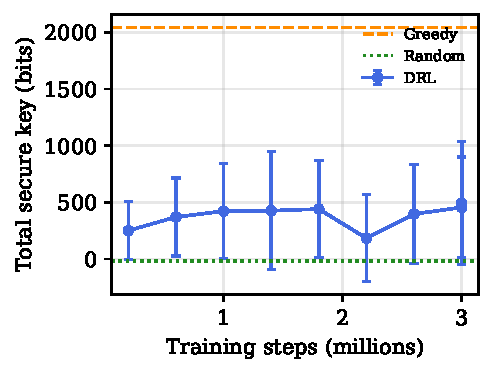
\includegraphics[width=\linewidth]{learning_curve.pdf}
    \caption{Learning curve (Realistic).}
    \label{fig:learning_curve}
  \end{subfigure}
  \hfill
  \begin{subfigure}{0.46\linewidth}
    \centering
    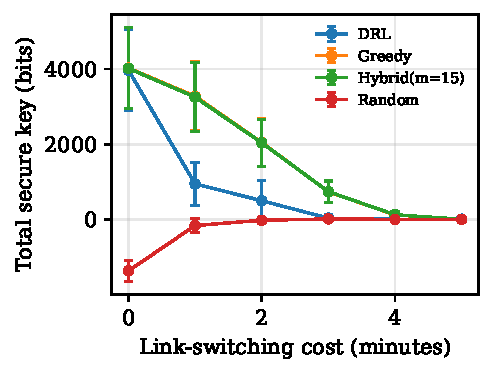
\includegraphics[width=\linewidth]{ablation_switching_cost.pdf}
    \caption{Switching-cost sensitivity.}
    \label{fig:ablation}
  \end{subfigure}
  \caption{Experimental results. (a) DRL performance in the Realistic scenario converges well before three million steps. (b) As the link-switching cost grows, Greedy and Hybrid degrade together and all policies collapse near $C = \CollapseCost$ minutes; the DRL agent stays below Greedy throughout. Error bars show one standard deviation over \Nseed{} seeds.}
  \label{fig:results}
\end{figure}

\textbf{Interpretation.} We attribute the Realistic gap to an overly conservative local optimum: the zero reward during setup forms an exploration barrier, and the agent learns to under-switch, holding a declining link too long and forgoing reconnections that Greedy seizes despite the latency. The ablation isolates the cause: at zero switching cost the DRL agent matches Greedy (Figure~\ref{fig:results}(b), \DRLstatM{} versus \GreDynM{}), so the failure is specific to cost-aware planning rather than to the scheduling task itself. The gap then widens monotonically as the cost grows.

\textbf{Reliability.} Beyond the mean shortfall, the learned policy is operationally unstable: in the Realistic scenario its per-seed return varies almost as much as its mean ($s_\pi \approx \mu_\pi$, Table~\ref{tab:results}), and individual 24-hour episodes range from near-zero to a few thousand bits, whereas Greedy is consistently strong. For an operational key-distribution network, this variance is itself disqualifying, independent of the average. The practical message is that a standard DRL algorithm is not a guaranteed path to superior performance when a strong domain heuristic exists, especially under penalties or delayed rewards; closing the gap likely requires mechanisms beyond vanilla PPO, such as curiosity-driven exploration, hierarchical control, or tighter learning-plus-heuristic integration.

\textbf{Limitations.} Our conclusions are specific to a single-satellite, five-station setting with one algorithm and a flat MLP policy. The gap may thus partly reflect this architecture rather than a fundamental limit of learning-based scheduling, and need not generalize to multi-satellite constellations, multi-agent coordination, or long-horizon planning, where learning could show clearer advantages; we regard these as natural next steps.

\section{Conclusion}\label{sec:conclusion}
We presented a reproducible, multi-seed study of DRL for Sat-QKD scheduling under one identical physical objective. DRL learns the simpler regimes well but does not outperform a strong greedy heuristic once realistic switching costs are present, even after extensive training, and a cost-aware hybrid does not close the gap because most reconfigurations are geometry-forced. The work offers a benchmark and a cautionary case, pointing future work toward advanced exploration or hybrid designs for operational quantum networks.

\bibliographystyle{ACM-Reference-Format}
\bibliography{references}

\end{document}
